\documentclass[aspectratio=149]{beamer}

\usepackage[utf8]{inputenc}
\usepackage[T1]{fontenc}

\usepackage[english]{babel}
\usepackage{amsmath}
\usepackage{cleveref}
\usepackage{amssymb}
\usepackage{mathtools}

%%Numbers, expectation
\newcommand{\N}{\mathbb{N}}
\newcommand{\E}{\mathbb{E}}
\renewcommand{\P}{\mathbb{P}}
\newcommand{\Var}{\mathbb{V}}
\newcommand{\R}{\mathbb{R}}
\newcommand{\D}{\mathcal{D}}
\newcommand{\B}{\mathcal{B}}
\newcommand{\Dh}{\D_h}
\renewcommand{\phi}{\varphi}
\newcommand*\diff{\mathop{}\!\mathrm{d}} % integral

%% mathoperator
\DeclareMathOperator*{\argmax}{arg\,max}
\DeclareMathOperator*{\argmin}{arg\,min}
\DeclareMathOperator*{\dom}{dom}
\DeclareMathOperator*{\sign}{sign}
\DeclareMathOperator*{\diag}{diag}

\DeclareMathOperator*{\Cov}{Cov}
\DeclareMathOperator*{\Cor}{Corr}
\DeclareMathOperator*{\Id}{Id}

%proximal operator
\newcommand{\prox}[3][]{\operatorname{prox}^{#1}_{#2}\left(#3 \right)}

\usepackage{xcolor}

%% sort citations by increasing number
\usepackage[sort,nocompress]{cite}

\usepackage{graphicx}% http://ctan.org/pkg/graphicx
\graphicspath{{../figures/}{../../figures}{../../memes}} %Setting the graphicspath
\usepackage{caption,subcaption}

\usepackage{tikz}
\usepackage{pgfplots}
\usetikzlibrary{backgrounds}
\usetikzlibrary{intersections}
\usepgfplotslibrary{fillbetween}

% \usepackage[right]{showlabels}


%%
\theoremstyle{plain}
\newtheorem{prop}{Proposition}[section]
\newtheorem{algo}{Algorithm}[section]
\newtheorem{assumption}{Assumption}
\theoremstyle{remark}
\newtheorem{remark}{Remark}[section]

% cref
\crefname{assumption}{Assumption}{Assumptions}
\crefname{equation}{}{}

\usepackage{autonum}

\usepackage{bm} %% bold math symbols

\usepackage{bbm} %% for \mathbbm{1}


% algorithmic environment
\usepackage{algorithm}
\usepackage[noend]{algpseudocode}

% for some reason this was required on one void linux installation (but not the other)
\usepackage{sansmathaccent}
\pdfmapfile{+sansmathaccent.map}

\author{Axel Böhm}

% shows which section we're in
\usetheme{Darmstadt}

% page number
\setbeamertemplate{footline}[frame number]
\setbeamercolor{page number in head/foot}{fg=gray}


% display things like onslide or visible already before but grayed out
\setbeamercovered{transparent}

% set the itemize item symbol as a diamond
\setbeamertemplate{itemize item}{$\diamond$}
% set the itemize subitem symbol as a triangle
\setbeamertemplate{itemize subitem}{$\blacktriangleright$}

% set the enumerate item symbol as a roman numbers
\setbeamertemplate{enumerate item}{(\roman{enumi})}


\author{Axel Böhm}

% shows which section we're in
\usetheme{Darmstadt}

% page number
\setbeamertemplate{footline}[frame number]
\setbeamercolor{page number in head/foot}{fg=gray}


% display things like onslide or visible already before but grayed out
\setbeamercovered{transparent}

% set the itemize item symbol as a diamond
\setbeamertemplate{itemize item}{$\diamond$}
% set the itemize subitem symbol as a triangle
\setbeamertemplate{itemize subitem}{$\blacktriangleright$}

% set the enumerate item symbol as a roman numbers
\setbeamertemplate{enumerate item}{(\roman{enumi})}


\usepackage{booktabs}

\title{Coordinate descent}
\date{\today}

\begin{document}
\maketitle
\frame{\tableofcontents}


\section{Introduction}%


\begin{frame}
  \frametitle{Coordinate Descent}
  \textcolor{blue}{Goal:} Find $x^* \in \R^d$ minimizing $f(x)$.

  \begin{figure}[ht]
    \centering
    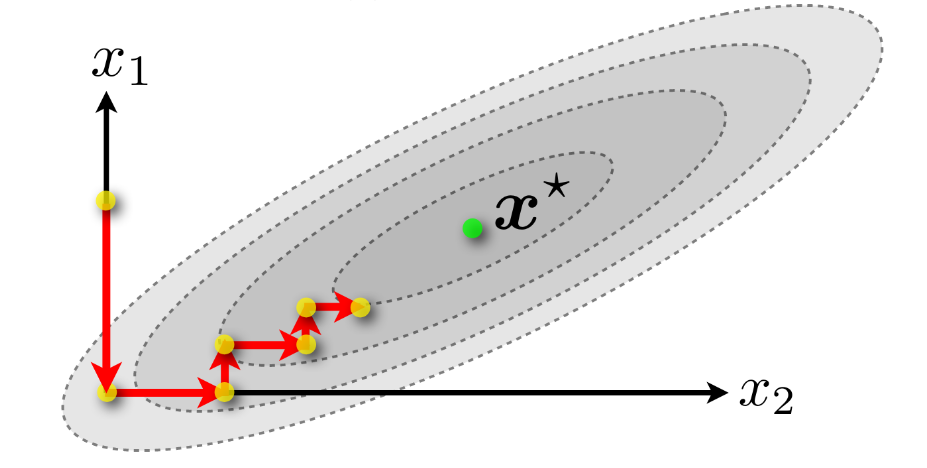
\includegraphics[width=\textwidth,height=\textheight,keepaspectratio]{coordinate_descent}
    \caption{\label{fig:label} }
  \end{figure}
\end{frame}

\begin{frame}
  \frametitle{Coordinate Descent}
  Modify only one coordinate per step:
  \begin{block}{}
    \begin{center}
      select $i_k \in \{1, \dots, d\}$\\
      $x_{k+1} = x_k + \gamma e_{i_k}$
    \end{center}
  \end{block}
  where $e_i$ is the $i$-th unit basis vector.
  Two main variants:
  \begin{itemize}
    \item \textcolor{blue}{Gradient-based stepsize:}
          \begin{equation}
            x_{k+1} = x_k - \frac1L \nabla_{i_k}f(x_k) e_{i_k}
          \end{equation}
    \item \textcolor{blue}{Exact coordinate minimization:} \\
          Solve the scalar problem $\argmin_{\gamma\in \R} f(x_k + \gamma e_{i_k})$.
          \begin{itemize}
            \item \textit{hyperparameter free}
          \end{itemize}
  \end{itemize}
\end{frame}

\begin{frame}
  \frametitle{Randomized Coordinate Descent}

  \textit{How to choose the coordinate?}

  \begin{block}{}
    \begin{center}
      select $i_k \in \{1, \dots, d\}$ uniformly at random\\
      $x_{k+1} = x_k + \gamma e_{i_k}$
    \end{center}
  \end{block}
  \vspace{1cm}
  \begin{itemize}
    \item \textcolor{blue}{Faster convergence} than gradient descent\\
          (if coordinate step is $d$ times cheaper than full gradient step)
  \end{itemize}
\end{frame}

\begin{frame}
  \frametitle{Technical assumptions}

  \begin{block}{}
    \textcolor{blue}{Coordinate-wise smoothness:}
    \begin{equation}
      f(x + \gamma e_i) \le f(x) + \gamma \nabla_i f(x) + \frac{L}{2}\gamma^2, \quad \forall x \in \R^d, \forall \gamma \in \R, \forall i \in [d]
    \end{equation}
  \end{block}
  Is equivalent to coordinate-wise Lipschitz gradient:
  \begin{equation}

  \end{equation}

  \begin{itemize}
    \item
    \item
  \end{itemize}

\end{frame}


\end{document}
